\documentclass{ctexart}
%
%页眉页脚
\usepackage{geometry}
\geometry{left=2.5cm,right=2.5cm,top=2.5cm,bottom=2.5cm}
\usepackage{xcolor}
\usepackage{graphicx}
\usepackage{amsmath}
\usepackage{url}
\usepackage{enumerate}
\usepackage{subfigure}
\usepackage{listings}
\usepackage[colorlinks,linkcolor=black]{hyperref}%书签
\usepackage{fancyhdr}

\fancyhead[R]{\thepage}%这是奇数页右页眉、偶数页左页眉
\fancyhead[L]{}
\chead{全球导航卫星系统基础}%这是中间页眉
\pagestyle{fancy}
\lstset{
    extendedchars=false, %解决代码跨页时,章节标题,页眉等汉字不显示的问题
    xleftmargin=1.5em,xrightmargin=1.5em, aboveskip=1em, %设置边距
    language=Matlab,
    basicstyle = \footnotesize,
    breaklines,
    captionpos = t,
    commentstyle = \color[rgb]{0,0.5,0},
    frameshape = {RYRYNYYYY}{yny}{yny}{RYRYNYYYY},
    keywordstyle = \color{blue}\bfseries,
    numbers = left,
    numberstyle = \tiny\color[rgb]{0.5,0.5,0.5},
    showstringspaces = false,
    stringstyle = \color[rgb]{0.58,0,0.82},
    tabsize = 4,
    title = \lstname
}
%中文
\usepackage{xeCJK}
%字体设置
\usepackage{enumitem}
\usepackage{indentfirst}
\setlength{\parindent}{2em}%首行缩进
\renewcommand\thesubsection{\alph{subsection}}
\renewcommand\thesubsubsection{\alph{subsubsection}}
\CTEXsetup[format={\Large\bfseries}]{section}

\title{第二次大作业P2:PVT解算}
\author{聂浩(2013011280)}
\date{\today}
\begin{document}
\maketitle
\section{单系统定位:自己实现一种定位解算算法,分别利用GPS、北斗的数据文件计算用户的位置与速度。通过查阅地图,看看用户的位置在哪里?}

    \subsection{单GPS}
    中国境内大部分地图采用的为GCJ02火星坐标系,而百度地图使用的为BD09坐标系,而所提供的GPS数据为基于WGS84的ECEF坐标系。

    本次大作业中首先完成的是对于以上坐标系的相互转换\footnote{这里参考了相关代码\url{https://github.com/wandergis/coordTransform_py}}以及ECEF与LLH坐标的转换\footnote{使用matlab 2015b自带函数},具体可见co\_trans\footnote{执行本作业中的程序需要将co\_trans文件夹添加到路径中,或者将其中的文件拷出}中的文件。

    随后进行PVT解算,由于本作业中没有提供T的数据,所以这里仅仅进行PV解算,代码如下
    \lstinputlisting{gps.m}
    \lstinputlisting{pvt.m}

    计算得到的位置点如图\ref{gps}\footnote{该图为调用百度地图API绘制,相关代码见map/gps.html,请使用Chrome浏览器打开},速率如图\ref{v_gps},单位为m/s
\begin{figure}
    \centering
    % Requires \usepackage{graphicx}
    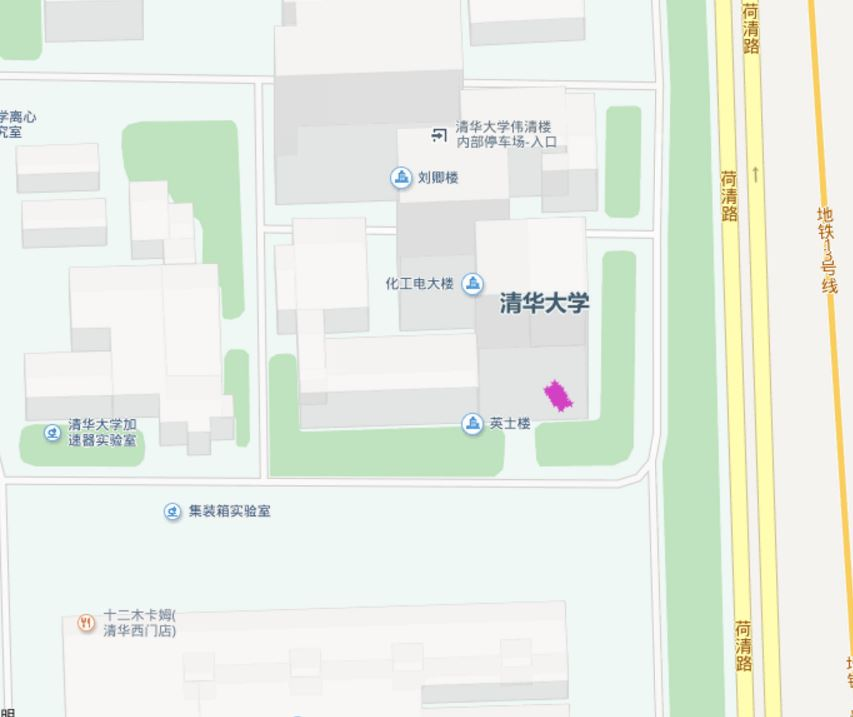
\includegraphics[width=0.8\textwidth]{pic/gps.jpg}\\
    \caption{GPS定位结果}
    \label{gps}
\end{figure}
\begin{figure}
    \centering
    % Requires \usepackage{graphicx}
    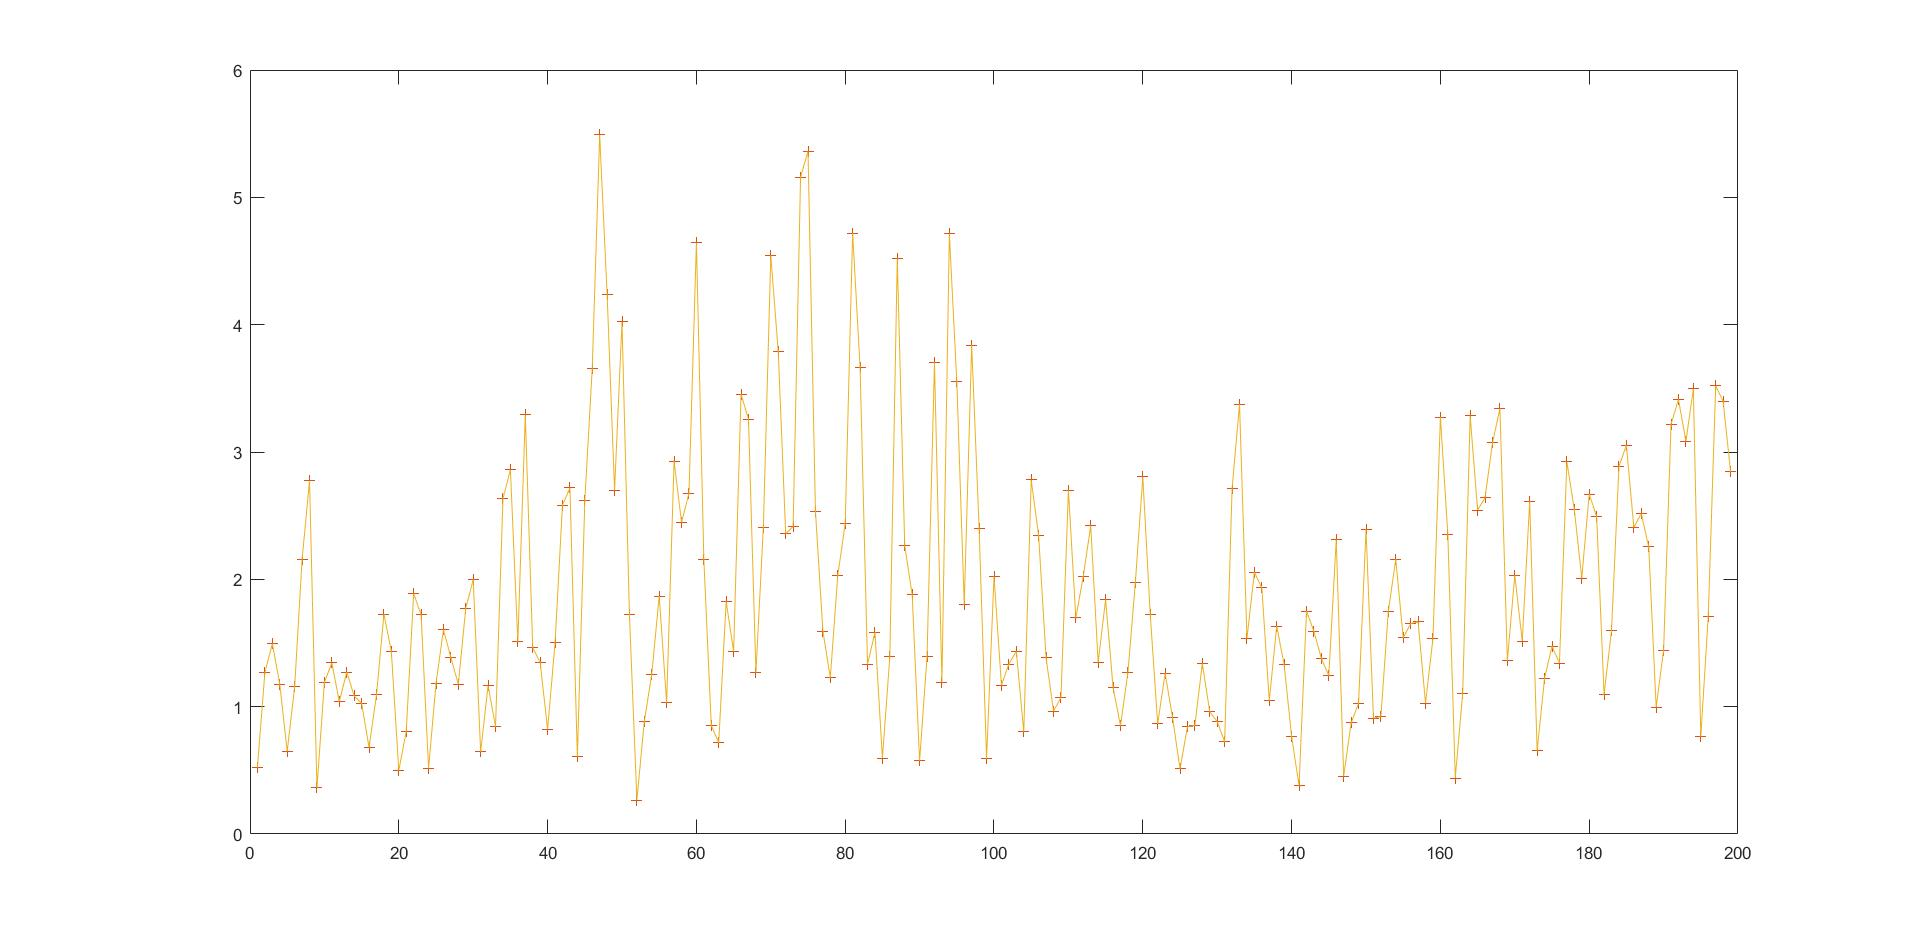
\includegraphics[width=0.8\textwidth]{pic/v_gps.jpg}\\
    \caption{GPS定位速率}
    \label{v_gps}
\end{figure}


\subsection{单北斗} 根据相关参考文献,“WGS84坐标与CGCS2000坐标的差值在cm级范围内”\footnote{\texbf{WGS84和CGCS2000坐标转换研究}彭小强},所以这里直接用WGS84坐标系对北斗信号进行结算,相关代码见附录所附beidou.m。
    计算得到的位置点如图\ref{beidou},速率如图\ref{v_beidou},单位为m/s
\begin{figure}
    \centering
    % Requires \usepackage{graphicx}
    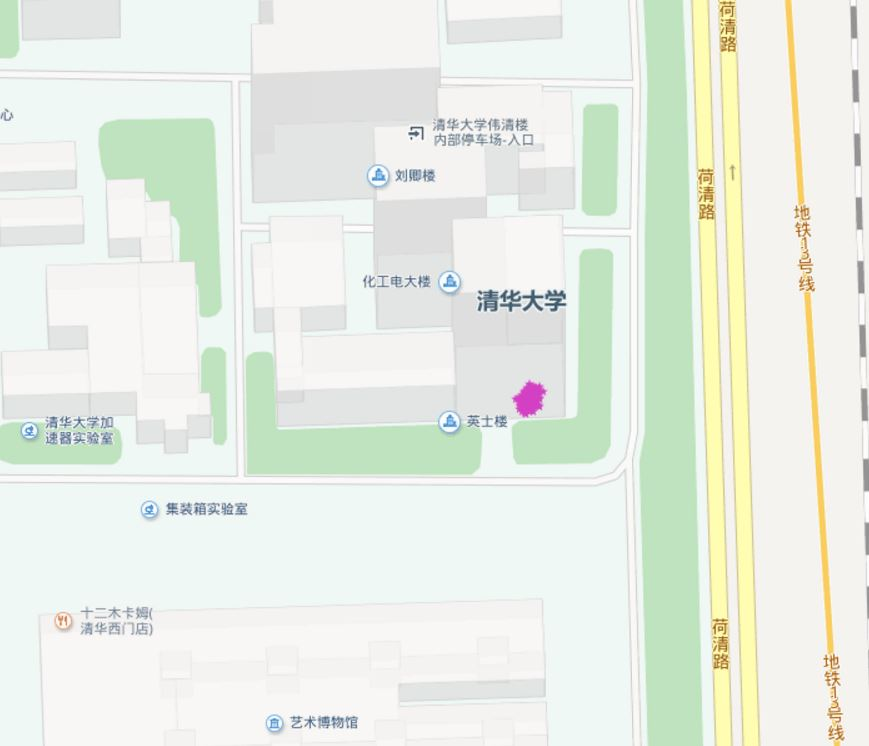
\includegraphics[width=0.8\textwidth]{pic/beidou.jpg}\\
    \caption{北斗定位结果}
    \label{beidou}
\end{figure}
\begin{figure}
    \centering
    % Requires \usepackage{graphicx}
    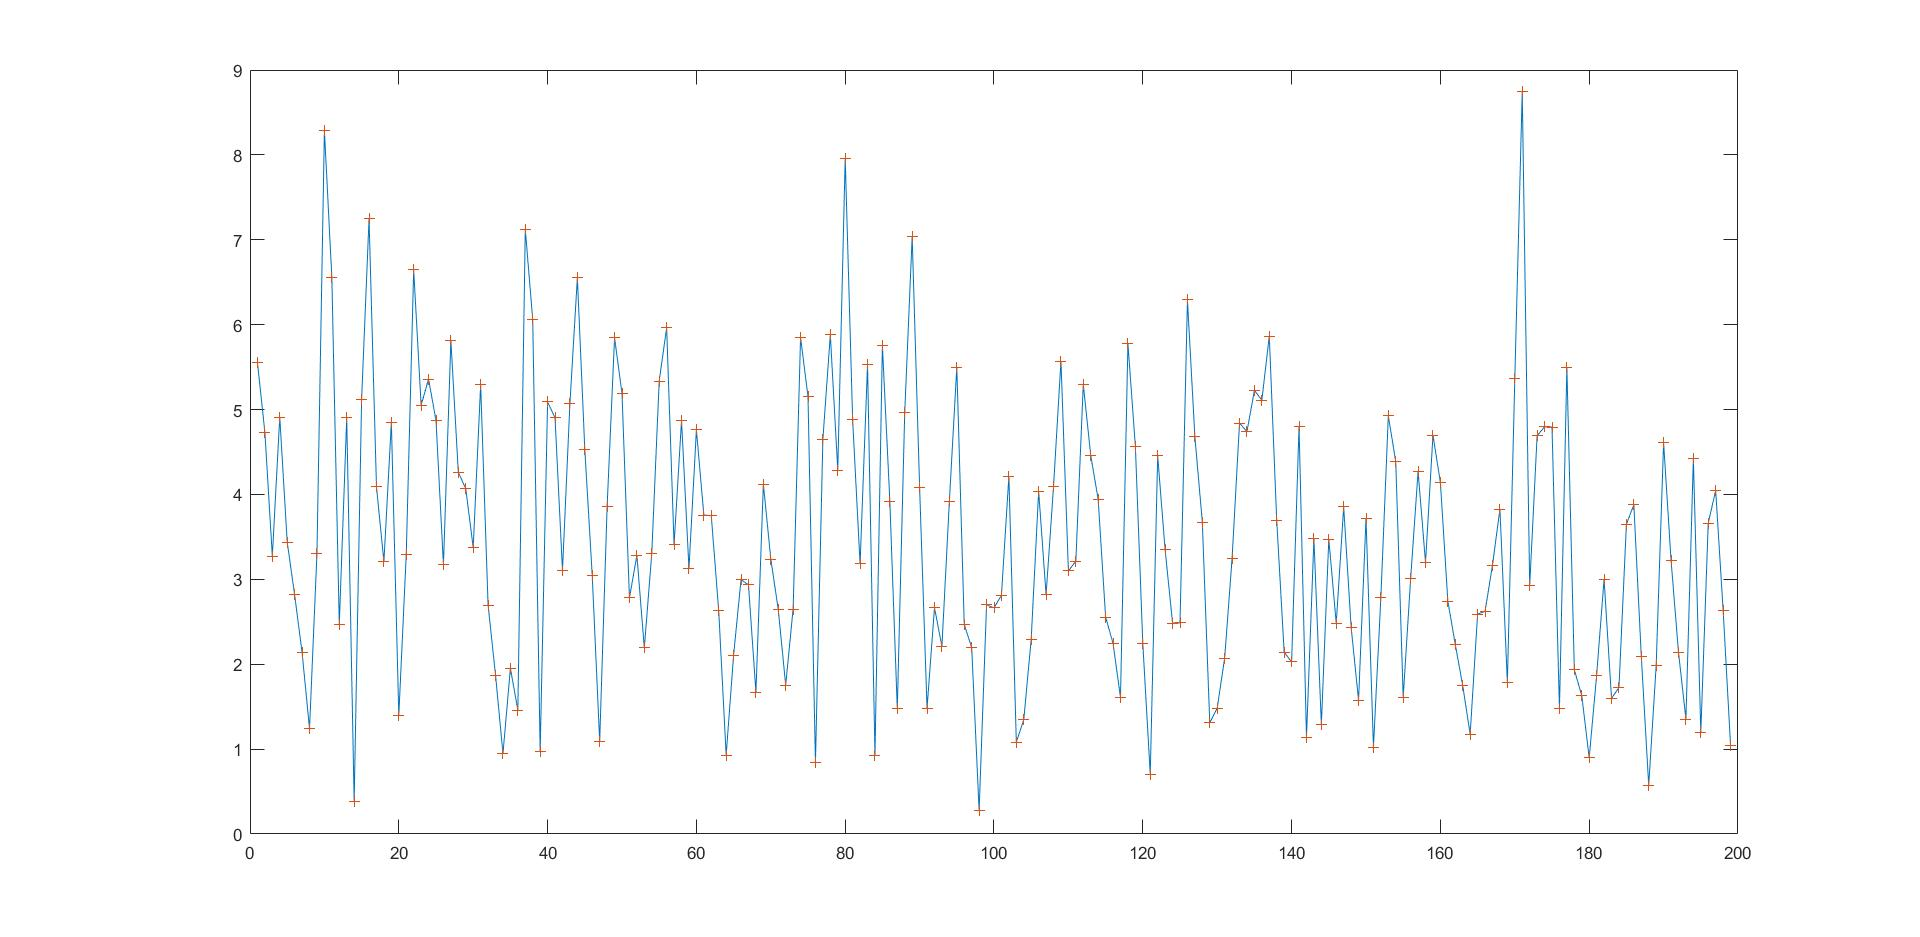
\includegraphics[width=0.8\textwidth]{pic/v_beidou.jpg}\\
    \caption{北斗定位速率}
    \label{v_beidou}
\end{figure}

\section{	联合定位(多模接收):自己实现一种定位解算算法,联合使用GPS、北斗的数据文件计算用户的位置与速度。并将该定位结果与单独使用GPS、北斗时的定位解算结果进行比较?给出你的结论?}
根据上一问的结论可以看出,200个定位点之间的距离非常小,即整个定位过程中用户几乎没有移动,这里将北斗的7颗卫星信息直接附在GPS信号之后,即PVT解算中以14颗星进行解算。代码见附录merge.m
    计算得到的位置点如图\ref{merge},速率如图\ref{v_merge},单位为m/s,从定位图可以看出,多模接受得到的200个定位点更加集中,可见其精度更高。
\begin{figure}
    \centering
    % Requires \usepackage{graphicx}
    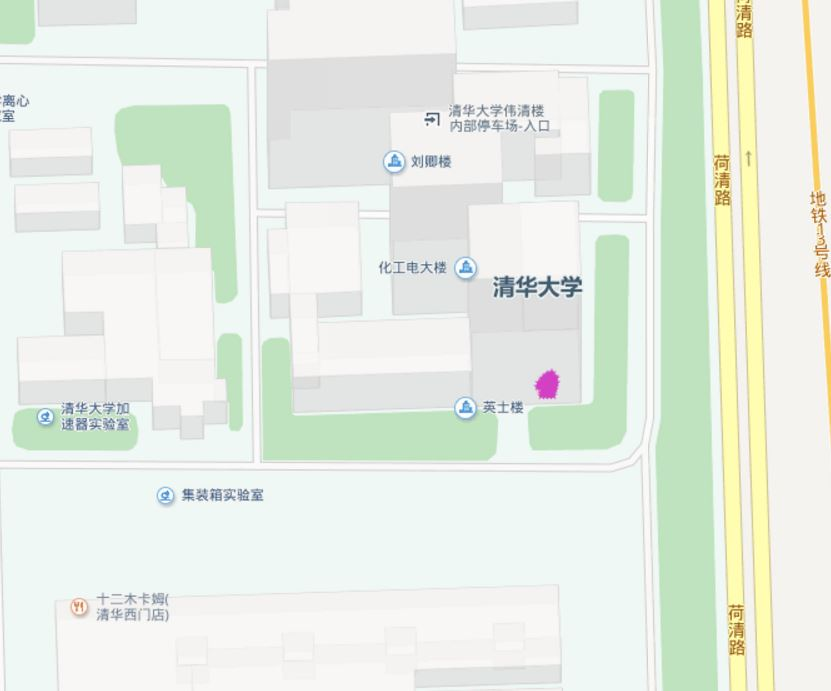
\includegraphics[width=0.8\textwidth]{pic/merge.jpg}\\
    \caption{联合定位结果}
    \label{merge}
\end{figure}
\begin{figure}
    \centering
    % Requires \usepackage{graphicx}
    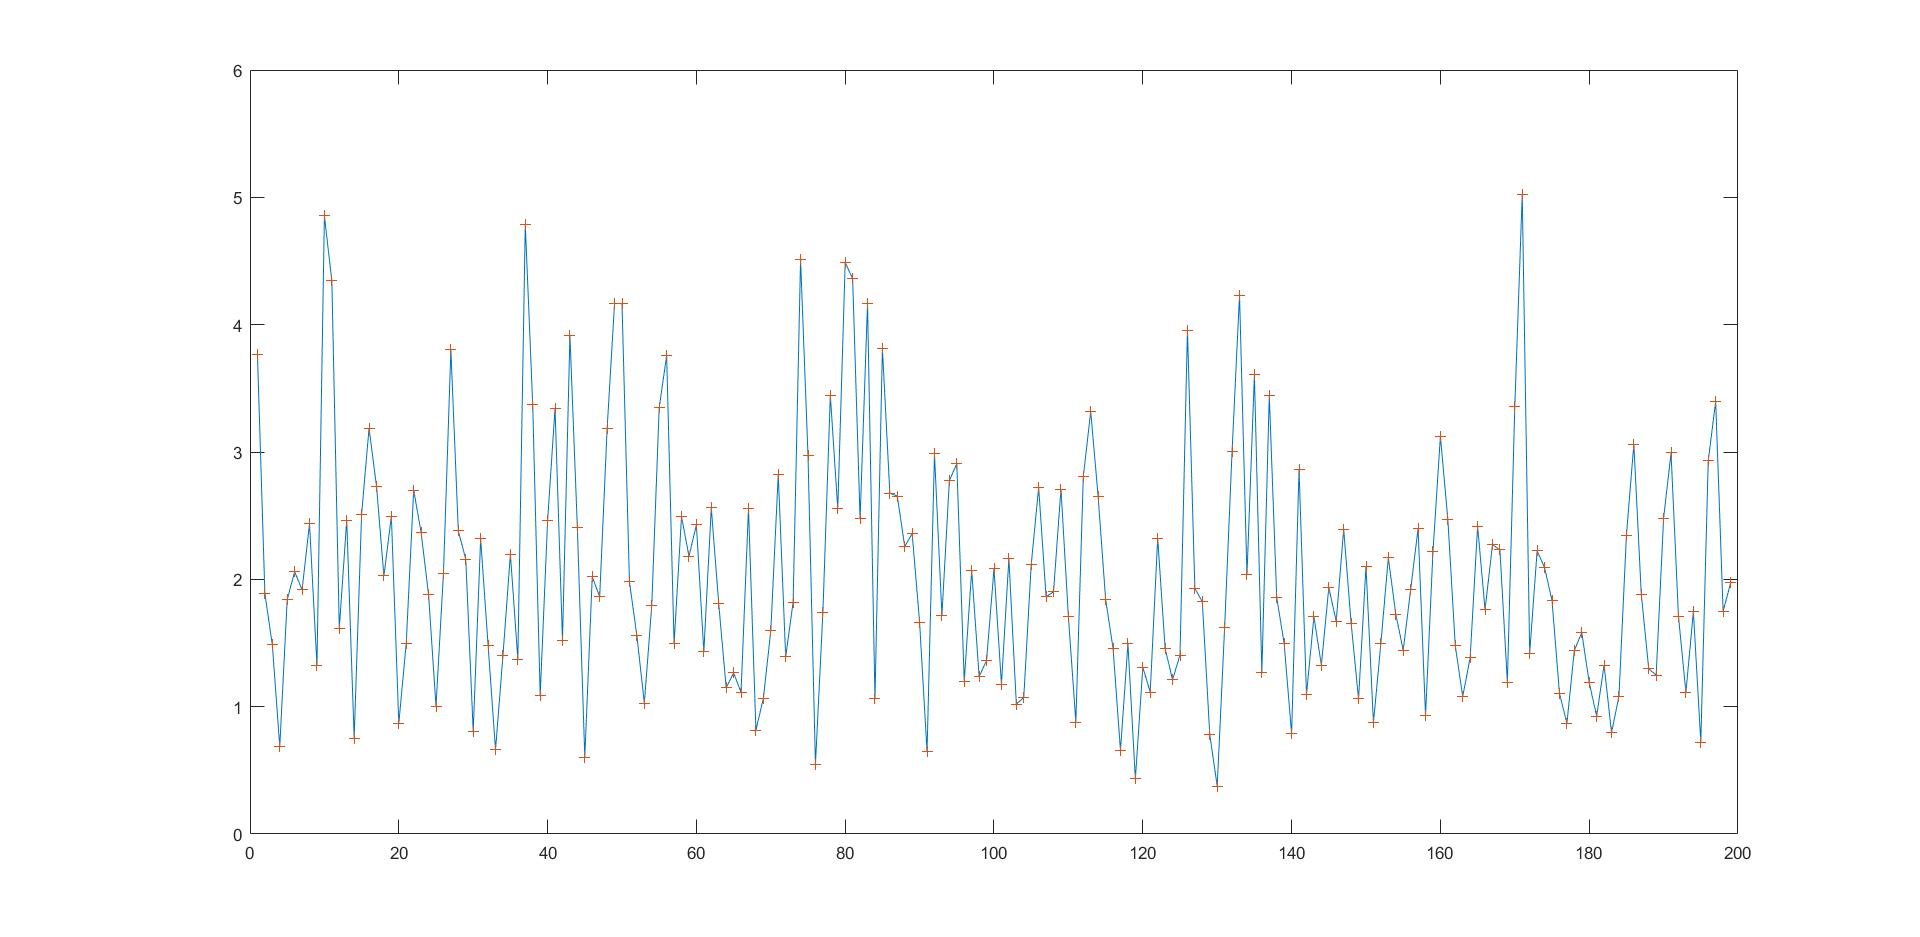
\includegraphics[width=0.8\textwidth]{pic/v_merge.jpg}\\
    \caption{联合定位速率}
    \label{v_merge}
\end{figure}

\section{	在导航系统使用中,一般希望收到的卫星数越多越好,即希望采用更多的卫星来进行定位解算,这也是目前国际上开发新卫星导航系统的出发点之一。在此,试改变GPS、北斗可用卫星数,然后再定位,并比较定位解算结果的变化?给出你的结论?}
只是用GPS的前五颗卫星数据进行PVT解算,相关代码见附录reduce.m.

所得结果如图\ref{reduce},速率如图\ref{v_reduce},单位为m/s,从定位图可以看出,卫星减少后定位的区域变大,可见会出现更大的误差。
\begin{figure}
    \centering
    % Requires \usepackage{graphicx}
    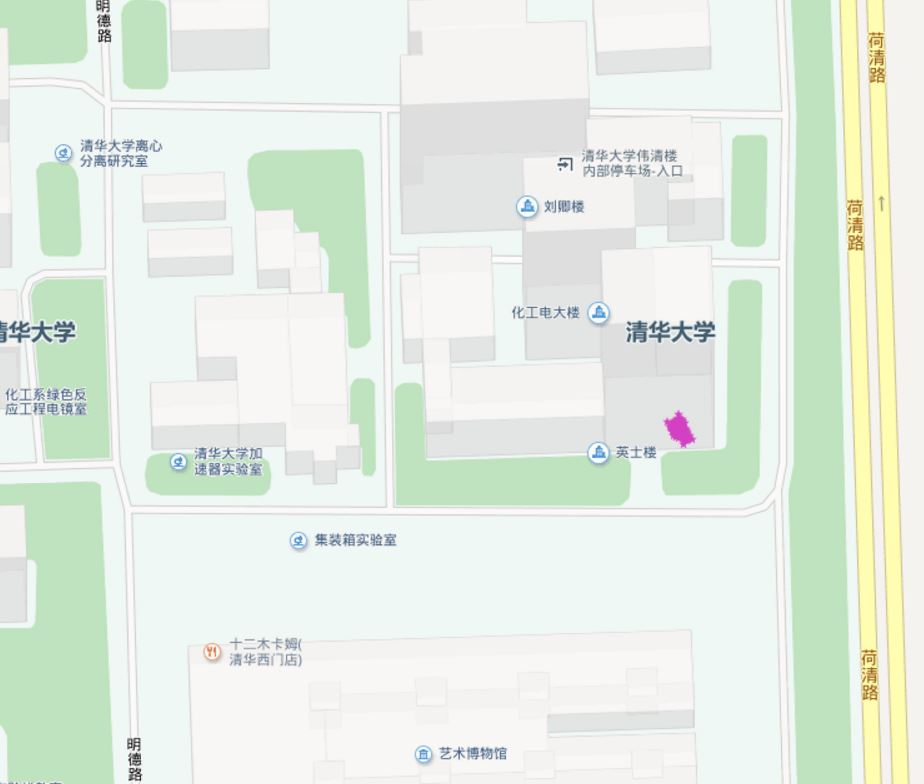
\includegraphics[width=0.8\textwidth]{pic/reduce.jpg}\\
    \caption{减少卫星后GPS定位结果}
    \label{reduce}
\end{figure}
\begin{figure}
    \centering
    % Requires \usepackage{graphicx}
    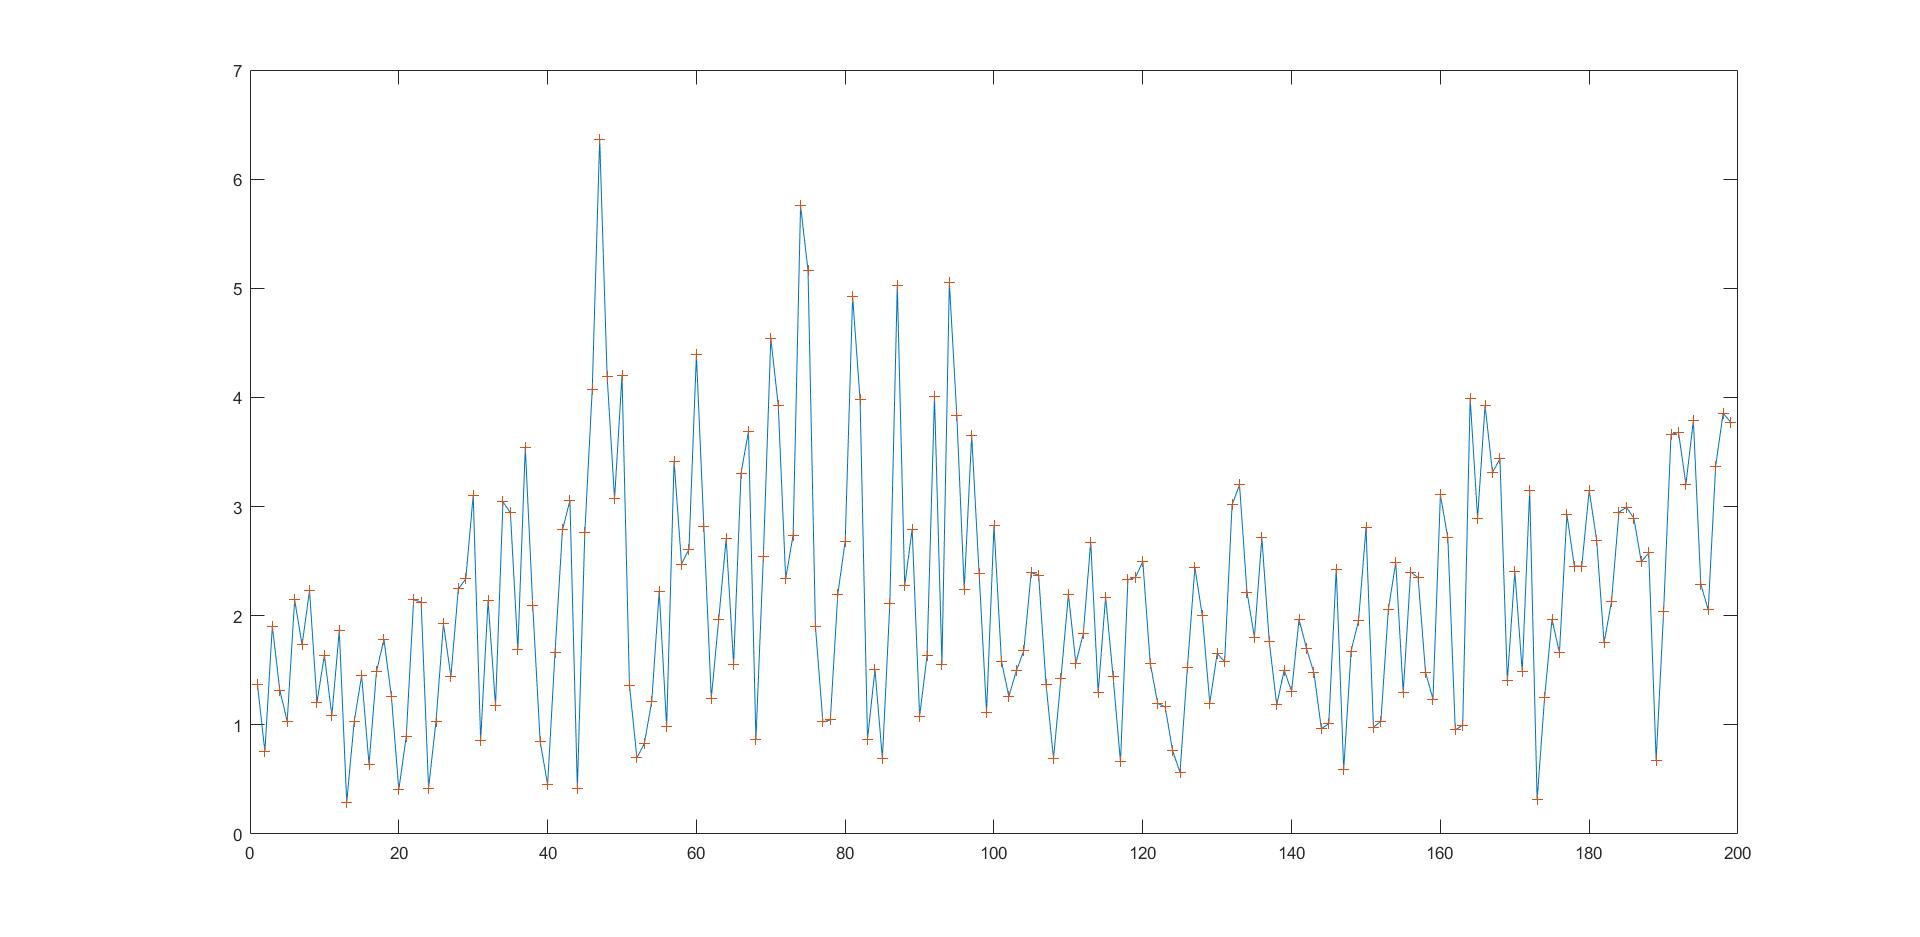
\includegraphics[width=0.8\textwidth]{pic/v_reduce.jpg}\\
    \caption{减少卫星后GPS定位速率}
    \label{v_reduce}
\end{figure}
\section{附录}
\lstinputlisting{beidou.m}
\lstinputlisting{merge.m}
\lstinputlisting{reduce.m}
\end{document}
